\section{Collections}

In this section we will introduce the \textit{Java Collections API}. In doing so we will discuss three broad classifications of data structures provided by the API:
\begin{enumerate}
    \item Sequential-based
    \item Dictionary-based
    \item Set-based
\end{enumerate}
Note that our discussion is not all-inclusive of every data structure in the API, but we present those that we feel are most valuable to this course.

\subsection*{Sequential-Based Data Structures}
We categorize data structures that have an ordering over the natural numbers as \textit{sequential-based}. That is, each element has an index where it ``lives'' for its lifetime. Each index is, similar to standard arrays, numbered from zero to the size of the collection minus one. Let us now take a dive into these different collections.
\subsubsection*{\ttt{ArrayList} Class}
Arrays are fixed-size data structures; once they are initialized, they cannot, themselves, be resized. A solution to this problem is to create a new array $A'$ of the same type with a new size and copy the elements from the old array to $A'$. Doing so is not difficult but cumbersome to repeatedly implement. Consider a situation in which the number of elements to store is unknown at compile-time. We, therefore, cannot use an array without repeated resizing. The correct and colloquial solution involves the \ttt{ArrayList} class.

First, however, let us see how we might go about implementing a \textit{dynamic array}, called a \textit{list}. using only methods. Suppose we want to store positive integers in this list. We also want to be able to add, set, and retrieve elements at a specified index. We will continue to work with arrays for the time being to demonstrate what goes wrong with this ideology, and then to understand the power of the \ttt{ArrayList}.

We need a few methods to solve this problem: \ttt{makeList}, \ttt{addToList}, \ttt{getFromList}, and \ttt{setInList}. At the end of the day, we want the programmer who uses these methods to not worry about resizing the array themselves; the logic within handles the dirty work.

To better relate to the \ttt{ArrayList} class implementation, we will write two versions of the \ttt{makeList} method: one that receives an initial size and one that does not. Designing two methods of the same name that receive different parameter types/quantities is known as \textit{method overloading}\index{method overloading}, and we will see this further in our discussion on \textit{classes}. \ttt{makeList} returns an array of integers instantiated to the given size, or a base size of ten elements in the method that does not receive a parameter. Note that, inside of the \ttt{makeList} method that does not receive a parameter, we invoke \ttt{makeList(10)} so as to not repeat ourselves.

\begin{cl}[]{Dynamic Integer Array Method ``Constructors''}
\begin{lstlisting}[language=MyJava]
class DIntArray {

  /**
   * Creates an array of the given size.
   */
  static int[] makeList(int size) {
    int[] array = new int[size];
    for (int i = 0; i < array.length; i++) {
      array[i] = -1;
    }
    return array;
  }

  /**
   * Creates an array with ten spaces.
   */
  static int[] makeList() {
    return makeList(10);
  }
}
\end{lstlisting}
\end{cl}

We now want a method that will add a value to a given ``list'' in this fashion. In particular, we know that indices whose elements are $-1$ correspond to ``free/available'' slots for the next value to-be added. The thing is, there is more to consider than just replacing the first-found instance of $-1$ with the desired value. We need to ensure that room exists for this new value; i.e., whether or not there is a $-1$ to begin with. As such, we should write a local helper method that returns a resized list with the values copied over from the old list; the only difference being a doubling in element capacity. Then, inside \ttt{addToList}, we check to see if we were able to properly insert $v$ into the list and, if not, we resize and make a recursive call to \ttt{addToList}.\footnote{We could use \ttt{Arrays.copyOf}, but it is important to understand \textit{how} the copying occurs.} Regarding performance and memory usage, this is not an optimal solution since we could simply add $v$ to index $|A|$ of the new array $A'$, since we know $|A'| = |A|$.

\begin{cl}[]{Adding Value into Dynamic Array Tests}
\begin{lstlisting}[language=MyJava]
import static Assertions.assertAll;
import static Assertions.assertArrayEquals;
import static DIntArray.makeList;
import static DIntArray.add;

class DIntArrayTester {

  @Test
  void addTest() {
    int[] arr1 = makeList(5);
    int[] arr2 = addToList(arr1, 20);
    int[] arr3 = addToList(arr2, 350);
    assertArrayEquals(new int[]{20, -1, -1, -1, -1}, arr2);
    assertArrayEquals(new int[]{20, 350, -1, -1, -1}, arr3);
  }
}
\end{lstlisting}
\end{cl}

\begin{cl}[]{Resize Array Method Implementation}
\begin{lstlisting}[language=MyJava]
class DIntArray {

  /**
   * Doubles the capacity of a list, returning a 
   * new list with the old elements copied over.
   */
  private static int[] resize(int[] list) {
    int[] newList = new int[list.length * 2];
    for (int i = 0; i < list.length; i++) {
      newList[i] = list[i];
    }
    return newList;
  }
}
\end{lstlisting}
\end{cl}

\begin{cl}[]{Adding Value into Dynamic Array Implementation}
\begin{lstlisting}[language=MyJava]
class DIntArray {

  /**
   * Adds a value to the next-available spot in the list.
   * We define next-available as the first -1 we find from the left.
   */
  static int[] addToList(int[] list, int v) {
    boolean added = false;
    int[] newList = makeList(list.length);
    for (int i = 0; i < list.length; i++) {
      // If we haven't inserted the value yet and we found
      // a free slot, insert it and mark added as true.
      if (list[i] == -1 && !added) {
        newList[i] = v;
        added = true;
      } else {
        // Otherwise, just copy over the old value.
        newList[i] = list[i];
      }
    }
    if (!added) { return addToList(resize(newList), v); } 
    else { return newList; }
  }
}
\end{lstlisting}
\end{cl}

We have two methods to go: \ttt{getFromList} and \ttt{setInList}. The former retrieves an element at a given index and the latter replaces the element at a given index. Both methods receive an index $i$ that must be in-bounds, where in-bounds refers to not only the bounds of the array, i.e., neither negative nor exceeding the length of the list, but also the logical indices. The \textit{logical indices} of a list are the indices in which elements exist. For our purposes, these indices are from zero up until and excluding the first instance of $-1$. We will also write a helper method that retrieves the index of the first ``free'' slot of a list, i.e., the first occurrence of $-1$.

\begin{cl}[]{``Get From List'' Dynamic Array Implementation}
\begin{lstlisting}[language=MyJava]
class DIntArray {

  static int getFromList(int[] list, int idx) {
    int upperBound = getFirstFreeSlot(list);
    if (idx < 0 || idx >= upperBound) {
      return -1;
    } else {
      return list[idx];
    }
  }

  private static int getFirstFreeSlot(int[] list) {
    for (int i = 0; i < list.length; i++) {
      if (list[i] == -1) { return i; }
    }
    return -1;
  }
}
\end{lstlisting}
\end{cl}

\begin{cl}[]{``Set In List'' Dynamic Array Implementation}
\begin{lstlisting}[language=MyJava]
class DIntArray {

  static int[] setInList(int[] list, int idx, int v) {
    int upperBound = getFirstFreeSlot(list);
    if (idx < 0 || idx >= upperBound) {
      return -1;
    } else {
      return list[idx];
    }

    // Copy over old elements.
    int[] newList = makeList(list.length);
    for (int i = 0; i < list.length; i++) {
      if (i == idx) {
        newList[i] = v;
      } else {
        newList[i] = list[i];
      }
    }
    return newList;
  }
}
\end{lstlisting}
\end{cl}

It should be noted that our implementation is a \textit{functional list}, which means that the (old) passed list, in and of itself, is not altered. Rather, we create a new list with each successive modification.

So, the problems of relying only on methods become clear: we have no way of keeping track of when/where the last \textit{logical element} is located. By assuming an input of only positive integers, we can say that the first occurrence of a $-1$ marks the next-available spot to add a value. Sentinel indicators like these fall apart once we allow for different inputs, e.g., negative numbers. 

The Java \ttt{ArrayList} class is a dynamic list data structure, is our first look at a ``powerful'' data structure insofar as its capabilities are concerned. Additionally, it is the first class that incorporates \textit{parameterized types}. With arrays, we must specify the type upon declaration; the \ttt{ArrayList} class is \textit{generic} in the sense that it operates on any type, whether that is \ttt{Integer}, \ttt{String}, or anything else, making it an incredibly flexible data structure. 

What makes an \ttt{ArrayList} so convenient is the abstraction and encapsulation of the underlying data structure. Underneath these lies a primitive array that is resized whenever necessary, similar to our resizing method. Thankfully, us as the programmers need not to worry about its implementation, but understanding it is key to grasping just what makes it better than our previous approach of writing static methods that receive and return lists. First, like we said, our methods-based implementation of dynamic lists is restricted to one datatype, namely \ttt{int}, and also uses $-1$ as the ``sentinel.'' Conversely, \ttt{ArrayList} stores a number that references the next-available spot, meaning we do not need to waste time traversing the list for each and every instance of adding or modifying elements.

\begin{figure}[tp]
%\begin{wrapfigure}[25]{r}[0.75in]{0.55\textwidth}
  \small
  \begin{tcolorbox}[title=Java Array Lists]
    An \textit{ArrayList}\index{ArrayList} is a dynamically-sized data structure for storing elements.
    \vspace{2ex}
    % \hrule
    % \vspace{2ex}
  \begin{description}
    \item [\ttt{List<$T$> $A=$ new ArrayList<>()}] creates an \ttt{ArrayList} of type $T$ named~$A$.
    \item [\ttt{$A$.get$(i)$}] retrieves the element at index $i^{\text{th}}$ of $A$. We refer to this as position $i + 1$. 
    \item [\ttt{$A$.set$(i, v)$}] assigns $v$ to index $i$ of $A$.
    \item [\ttt{$A$.size$()$}] returns the number of logical elements in the list, i.e., the logical size.
    \item [\ttt{$A_1$.equals}$(A_2)$] returns whether or not the elements of $A_1$ are equal to the elements of $A_2$, using the \ttt{.equals} method implementation of $A_1$.
    \item [\ttt{$A$.toString$()$}] returns a string representation of the elements in $A$, separated by commas and enclosed by brackets.
    \item [\ttt{Collections.sort}$(A)$] performs an in-place sort of $A$, meaning the contents of $A$ are modified.
  \end{description}
\end{tcolorbox}
  \caption{Useful \ttt{ArrayList}-based Methods.}
  \label{fig:arraylists}
\end{figure}

To declare an \ttt{ArrayList} called $A$, we write the following, where $T$ is a class representing the type of elements contained within:
\begin{verbnobox}[\small]
List<T> A = new ArrayList<>();
\end{verbnobox}
This initializes a \ttt{List} $A$, but instantiates it as a new \ttt{ArrayList}.\footnote{The reason behind this \textit{polymorphic} choice will become apparent in subsequent chapters.} Notice that we do not specify the number of elements to store like we would an array. Indeed, because lists are dynamic in size, there is no need to specify a default. Java defaults the starting size of a newly-declared \ttt{ArrayList} to ten elements, although this can be changed by passing a size argument between the parentheses.
\begin{verbnobox}[\small]
List<T> A = new ArrayList<>(100);
\end{verbnobox}
You might be tempted to ask, ``Why might that be necessary?'', which is a great question. Remember that resizing an array depends on the number of pre-existing elements. Thus, the fewer resizes there are, the better, hence why we double the array capacity in our functional list implementation. If we know that we might have a lot of elements to add to the list from the start, it is a good idea to specify this as a parameter to the \ttt{ArrayList}. On average, adding a value to the end of an \ttt{ArrayList} is a \textit{constant cost}\index{constant cost}, or occurs instantaneously, because we know exactly where the next free spot is located. We cannot forget the time it takes to resize, however, so we declare that the \ttt{.add} method takes constant time with respect to \textit{amortized analysis}\index{amortized analysis}. In essence, sometimes we have to perform a resize-and-copy operation, but on average, we do not need to consider the cost thereof.

Like arrays, modifying elements in-place and retrieval also has a constant cost; the underlying data structure is an array after all. We retrieve a value at a given index using \ttt{.get}, and we replace an existing value at a given index using \ttt{.set}.

\example{If we instantiate an \ttt{ArrayList} of integers $\ttt{ls1}$, we can perform several operations to demonstrate our understanding.}
\begin{verbnobox}[\small]
List<Integer> ls1 = new ArrayList<>();
ls1.add(439);
ls1.add(311);
ls1.add(654);
ls1.add(523);
ls1.toString();  => {439, 311, 654, 523}
ls1.get(0);      => 439
ls1.set(1, 212);
ls1.add(677);
ls1.toString()   => {439, 212, 654, 523, 677}
\end{verbnobox}
Finally, we can remove an element, when given its index, using \ttt{.remove}. Be aware that removing elements is not as simple as adding. Suppose that, from the previous example, we invoke $\ttt{ls1.remove}(2)$, which removes the value $654$. We cannot simply have a slot/index with a missing value. So, Java compensates by shifting all values to the right of the removed value over by one.

\example{Consider a situation in which we have an \ttt{ArrayList} that contains $1,000,000$ arbitrary integers. If we continuously remove elements from the front of the list, we shift each and every value down by one index. Propagating this through all one million elements results in a hefty cost of $999,999 + 999,998 + \cdots + 3 + 2 + 1$ shifts. So, removing $n$ elements from the front of an \ttt{ArrayList} is representable as an equation of time $T$.}

\[
T(n) = (n - 1) + (n - 2) + (n - 3) + \cdots + 3 + 2 + 1
\]

We can collapse this into an arithmetic series from $1$ to $n-1$:

\begin{align*}
T(n) &= \sum_{i=1}^{n-1}{i}\\
     &= n\cdot \left(\dfrac{1 + n - 1}{2}\right)\\
     &= n\cdot \left(\dfrac{n}{2}\right)\\
     &= \dfrac{n^2}{2}
\end{align*}

Therefore, to remove $1,000,000$ elements from the front of an \ttt{ArrayList}, we need to perform roughly $1,000,000^2/{2}$ operations, which is an astronomical number, even for computers of today. Removing elements from other indices, excluding the rear, will incur similar, yet smaller, shifting cost penalties. As we will see later in this chapter, other data structures are significantly better choices if it is a desire to quickly poll elements from the front.

\example{We made a big deal about growing the underlying array when we run out of room to add new elements. We could ask a similar question about what to do when we, say, remove a ton of elements from a large list. If our list contains one million elements and we then clear the list, it makes little sense, at first glance, to have space allocated for one million non-existent values. Though, Java's implementation of \ttt{ArrayList} does not decrease the size of the backing array, preferring performance over memory usage. The reasoning behind this choice is straightforward: suppose we have an \ttt{ArrayList} of $500$ elements and we remove $250$ elements. Is it fair to decrease the size of the list by a factor of two? If so, what happens when we add one more element, totaling to $251$? We then have to grow the list, again, wasting valuable time.}

\example{Consider the following code. What does $s$ contain after execution?}
\begin{verbnobox}[\small]
List<Integer> ls1 = new ArrayList<>();
ls1.add(10);
List<Integer> ls2 = ls1;
ls2.add(20);
ls1.add(30);
String s = ls1.toString() + " " + ls2.toString();
\end{verbnobox}
Should you be unaware of aliasing, you might say it resolves to \ttt{"[10, 30] [20]"}. \textit{Aliasing}\index{aliasing} is a form of object-sharing. When allocating any type of \textit{object}, whether that object is an array, an \ttt{ArrayList}, a \ttt{String}, or something else, we assign a reference \textit{to} that object in memory via the variable declaration. That is, in the preceding code, \ttt{ls1} references the location, in memory, of an \ttt{ArrayList}. Correspondingly, when we declare \ttt{ls2} and assign to it \ttt{ls1}, we are not copying over the values from \ttt{ls1} into \ttt{ls2}; we are expressing that \ttt{ls2} should reference the same list as referenced by \ttt{ls1}. Therefore by asserting \ttt{ls2} as an alias of \ttt{ls1}, any modifications made to either is reflected when referencing the other. In this instance, $s$ resolves to \ttt{"[10, 20, 30] [10, 20, 30]"}

\example{Consider two methods \ttt{void increment(int x)}, which increments an integer variable, and \ttt{void increment(ArrayList<Integer> ls, int idx)}, which increments the value at a given index in a list of integers.}

\begin{verbnobox}[\small]
static void incrementInt(int x) {
  x = x + 1;
}

static void incrementList(ArrayList<Integer> ls, int idx) {
  ls.set(idx, ls.get(idx) + 1);
}
\end{verbnobox}

If we then pass a variable to the \ttt{incrementInt} method, we might expect the resulting value, outside of the method, to also be incremented. Unfortunately, that is not what happens--in the following code segment, we see that the primitive variable \ttt{y} remains unchanged outside of the method invocation. This happens because primitive values are \textit{passed by value}. In essence, methods receive a copy of the value, which means that the original variable is not modified, and the change made inside the scope of \ttt{incrementInt} is rendered useless. Compare this to what happens if we pass an \ttt{ArrayList<Integer>} to \ttt{incrementList}: we see that the change occurs both inside and outside the scope of the method body. Objects, e.g., \ttt{String}, \ttt{ArrayList}, arrays, and so forth, when supplied as arguments to methods, are passed by a paradigm that we will call \textit{pseudo-reference}.\footnote{The emphasis on calling this ``pseudo-reference'' is to provide an intuition for those readers who may know about true pass-by-reference, while satisfying those who want to angrily shout that Java is strictly pass-by-value.} Passing by pseudo-reference means to suggest that we are not truly passing the argument by reference, and this is correct. Objects in Java are still passed by value, but instead of creating a copy of the object, the object's corresponding hashcode is supplied to the method, which is roughly equivalent to a memory reference.\footnote{In Chapter~\ref{chapter-classes}, we will discuss object hashcodes in greater detail.} Therefore, any changes made to the value inside the method are reflected outside.

\begin{verbnobox}[\small]
int y = 5;
assertEquals(5, y);         // Assertion before increment.
incrementInt(y);
assertEquals(5, y);         // Assertion after increment.
\end{verbnobox}

\begin{verbnobox}[\small]
List<Integer> ls = new ArrayList<>();
ls.add(5);
assertEquals(5, ls.get(0)); // Assertion before increment.
incrementList(ls, 0);
assertEquals(6, ls.get(0)); // Assertion after increment.
\end{verbnobox}

\example{We have seen the repeated use of the \ttt{Integer} and \ttt{Double} classes when parameterizing the types for \ttt{ArrayList}, but what is the point? Could we not instead opt for \ttt{int} and \ttt{double}, as we have traditionally? The answer is a resounding no; we must take advantage of the luxury that is \textit{autoboxing} and \textit{autounboxing} through the \textit{wrapper classes}. The classes \ttt{Integer}, \ttt{Double}, as well as \ttt{Short}, \ttt{Byte}, \ttt{Long}, \ttt{Char}, and \ttt{Boolean} are classes that encapsulate, or box, a corresponding primitive value. Parameterized types only work with class types; primitive datatypes are disallowed. So, for instance, if we want to work with an \ttt{ArrayList} of \ttt{int} elements, we are required to use the \ttt{Integer} wrapper class in our type declaration. We can, of course, declare an \ttt{Integer} using the following overly-verbose syntax:}

\begin{verbnobox}[\small]
Integer x = new Integer(42);
int y = x.getValue(); // y = 42.
\end{verbnobox}

We explicitly wrap the primitive integer $42$ in $x$, which is of the \ttt{Integer} type, then unwrap its value to be stored in $y$. Manually wrapping and unwrapping primitives is tiresome and only introduces redundant code, hence why Java autoboxes and autounboxes as needed. For example, if we declare an \ttt{ArrayList} of \ttt{Integer} values, then add the primitive integer literal \ttt{42} to the list, Java will autobox the literal into its \ttt{Integer} wrapper. Going the other direction, if we want to iterate over the values in the list, we might use the enhanced-for loop. If Java did not support autounboxing, we would instead have to use \ttt{Integer} as opposed to \ttt{int} in the loop variable declaration. 

\begin{verbnobox}[\small]
ArrayList<Integer> al = new ArrayList<>();
al.add(42);
for (int e : al) {
  ...
}
\end{verbnobox}

\example{Testing is always important when writing programs, as this text has emphasized from the first page. Writing test cases for lists, naively, is cumbersome due to the repetition of \ttt{.add} method calls when populating the list. Instead, Java has the convenient \ttt{List.of} method, which receives any number of arguments. Let us see an example of this method.}

\begin{verbnobox}[\small]
// Old way:
List<Integer> ls1 = new ArrayList<>();
ls1.add(5);
ls1.add(40);
ls1.add(4);
ls1.add(42);

// New way:
List<Integer> ls2 = new ArrayList<>(List.of(5, 40, 4, 42));
\end{verbnobox}
Using \ttt{List.of} raises a question: does \ttt{List.of} only receive five integer arguments? What if I want to specify more than five, or less than five? The answer to this excellent question is that \ttt{List.of} is a \textit{variadic-argument method}\index{variadic-argument method}. Methods may be written to receive any number of arguments, which are then collapsed into a data structure that is traversable.

\example{Suppose we want to write a variadic method that computes the average of any number of given \ttt{double} values. Without variadic-argument methods, we must wrap these in a list or an array, then pass it to the method. Variadic arguments allow us to specify any desired number of arguments, and it is the responsibility of the method to interpret those values as a traversable data structure. So, to iterate over such a structure, we can use the enhanced-for loop.}

\begin{cl}[]{Variadic Argument \ttt{numAverage} Tester}
\begin{lstlisting}[language=MyJava]
import static Assertions.assertAll;
import static Assertions.assertEquals;
import static NumAverage.numAverage;

class NumAverageTester {

  @Test
  void numAverageTest() {
    assertAll(
      () -> assertEquals(0, numAverage()),
      () -> assertEquals(5.66, numAverage(5, 2, 10)),
      () -> assertEquals(55.2, numAverage(10, 65, 77, 81, 43)));
  }
}
\end{lstlisting}
\end{cl}

\begin{cl}[]{Variadic Argument \ttt{numAverage} Implementation}
\begin{lstlisting}[language=MyJava]
class NumAverage {

  /**
   * Computes the average of a sequence of provided integers.
   * @param variadic integers.
   * @return average if there is at least one number or zero otherwise.
   */
  static int numAverage(int ... nums) {
    double sum = 0;
    for (int e : nums) { sum += e; }
    return nums.length == 0 ? 0 : sum / nums.length;
  }
}
\end{lstlisting}
\end{cl}

\example{If we want to, say, specify that a method must receive at least two parameters, those being a \ttt{String} and an \ttt{int}, followed by zero or more \ttt{String} values, we may declare the first two parameters, then incorporate the variadic notation for the last. Doing so ensures that we pass the required parameters, but any thereafter are optional but variadic nonetheless.}

\begin{cl}[]{Requiring Parameters with Variadic Arguments}
\begin{lstlisting}[language=MyJava]
class RequiredVariadicParameters {

  static int doSomething(String s, int v, String ... vals) { (*;\textcolor{lightgray}{...};*) }
}
\end{lstlisting}
\end{cl}

\subsubsection*{\ttt{LinkedList} Class}
\textit{Linked lists}\index{linked list} remove us from the shackles of array-based data structures, in that, as their name implies, they are a series of \textit{nodes}\index{node}, or elements, linked together in a chain of sorts. These nodes need not be adjacent in memory, but rather reference each other to find what comes next in the chain/list. For instance, if we create a linked list, it has a \textit{front}\index{head}/\textit{head} element that always references, or points, to the first element in the list (upon initialization, the head refers to nothing). If we add a new element, the head now points to this first element. Subsequent additions to the list continue growing the chain and links. Namely, element 1 points to element 2, element 2 to 3, and so on. 

Elements have an associated index and value, but linked lists are not constrained to a static size even in the underlying implementation! So, we can add and remove links from the chain whenever we please with no shuffling of values around aside from links within the chain. Removing elements from the front of a linked list is constant time, and scales linearly with the number of elements in the list rather than a quadratic growth.

Of course, these advantages are not without their disadvantages. Reading and modifying elements are slower operations than the array counterparts since the elements are not contiguous blocks in memory. Recall that with an \texttt{ArrayList}, because elements are placed side-by-side in memory, we know the location of any arbitrary index in the array list by a multiplicative offset of the starting index and the ``byte-size'' of each element. Linked lists do not provide this guarantee and should not be treated as such. Adding and removing elements are ``faster'' in the sense that, as we stated, copying values over to a new array is out of the question. Because of this, though, we need to iterate/traverse through the list each time we wish to reference a provided index. The same goes for inserting elements into the list. Adding or removing elements from the front or rear of the list, on the other hand, are instant operations since we keep track of the first element of the list (and we can, similarly, keep track of the last!). Linked lists are also the backbone of many other data structures as we will soon see.
% The \textit{linked list} data structure belongs to the first of these three, similar to an array list. Unlike these, though, linked lists are not backed by an array. Rather, elements in a linked list are chained together, so to speak, via \textit{nodes}. Recall that with an \texttt{ArrayList}, because elements are placed side-by-side in memory, we know the location of any arbitrary index in the array list by a multiplicative offset of the starting index and the ``byte-size'' of each element. Linked lists do not provide this guarantee and should not be treated as such. \textit{Singly-linked list} nodes point to their successor nodes in the list. That is, the \textit{head} of the list points to the second element, which points to the third, and so on until we reach the end of the list whose ``next'' pointer is \texttt{null}. Accordingly, each node is located somewhere in memory that is unpredictable, meaning we lose the constant access time granted by array lists.
\begin{figure}[tp]
  \small
  \begin{tcolorbox}[title=Java Linked Lists]
    A \textit{LinkedList} is a node-based data structure where each element contains a link to its successor (and potentially predecessor).
    \vspace{2ex}
    % \hrule
    % \vspace{2ex}
  \begin{description}
    \item [\ttt{List<$T$> $A=$ new LinkedList<>()}] creates a \ttt{LinkedList} of type $T$ named~$A$.
    \item [\ttt{$A$.get$(i)$}] retrieves the element at index $i^{\text{th}}$ of $A$. We refer to this as position $i + 1$. 
    \item [\ttt{$A$.set$(i, v)$}] assigns $v$ to index $i$ of $A$.
    \item [\ttt{$A$.size$()$}] returns the number of logical elements in the list, i.e., the logical size.
  \end{description}
\end{tcolorbox}
  \caption{Useful \ttt{LinkedList}-based Methods.}
  \label{fig:linkedlists}
\end{figure}


\subsubsection*{\ttt{Stack} Class}
\begin{figure}[tp]
%\begin{wrapfigure}[25]{r}[0.75in]{0.55\textwidth}
  \small
  \begin{tcolorbox}[title=Java Stacks]
    A \textit{Stack} is a last-in-first-out (LIFO) data structure where each element is linked to the element immediately below. 
    \vspace{2ex}
    % \hrule
    % \vspace{2ex}
  \begin{description}
    \item [\ttt{Stack<$T$> $S=$ new Stack<>()}] creates a \ttt{Stack} of type $T$, named $S$.
    \item [\ttt{$S$.peek$()$}] returns, but does not remove, the top element of $S$.
    \item [\ttt{$S$.pop$()$}] returns and removes the top element of $S$.
    \item [\ttt{$S$.push$(e)$}] pushes $e$ to the top of $S$, making $e$ the element on the top of the stack.
    \item [\ttt{$S$.size$()$}] returns the number of logical elements in the stack.
  \end{description}
\end{tcolorbox}
  \caption{Useful \ttt{Stack}-based Methods.}
  \label{fig:stacks}
\end{figure}
Imagine you are washing dishes, by hand, at the kitchen sink. These dishes are assorted in a single stack to your left. A dish cannot be removed from anywhere but the top of the stack because displacement anywhere else will destroy the stack. Additionally, further imagine that people are, to your dismay, adding more dishes to the stack. Again, dishes cannot be added anywhere else but the top of the stack. 

The \textit{stack}\index{stack} data structure is as simple as it sounds---a collection of elements that operate on the principle of last-in-first-out, or LIFO\index{last-in-first-out}. In other words, the last thing that we enter is the first thing removed. Stack implementations contain at least the following operations: \textsc{pop}\index{pop} and \textsc{push}\index{push}, where the former removes the top-most element from the stack (if one exists), and the latter adds a new element to the top of the stack. There may also exist an operation to view, but not remove, the top-most element via \textsc{peek}\index{peek}. 

Stacks have the advantages of instant insertion and removal times but are obviously not as flexible as an array or linked list. A practical example of a stack data structure would be an ``undo'' function in a document-editing program---whenever an action is made, it is pushed to an event stack. An ``undo'' event would resemble popping an action off this stack. We illustrate this concept in Figure~\ref{fig:stackundo}.

\begin{figure}[ht]
\begin{center}
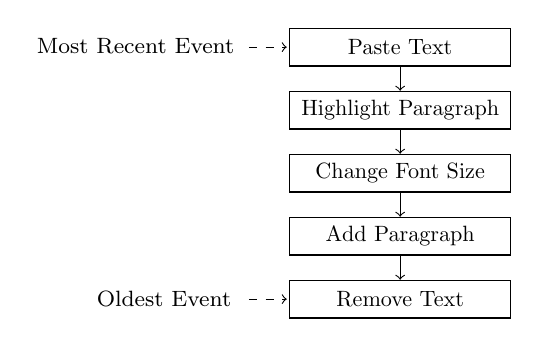
\begin{tikzpicture}[
  scale=.8,
  stacknode/.style={rectangle, draw, minimum width=1.5cm, minimum height=0.6cm, minimum width=3.5cm, text centered,scale=.8},
  dashedarrow/.style={->, dashed}
]

% Stack nodes
\node[stacknode] (top) at (0, 0) {Paste Text};
\node[stacknode] (node1) at (0, -1) {Highlight Paragraph};
\node[stacknode] (node2) at (0, -2) {Change Font Size};
\node[stacknode] (node3) at (0, -3) {Add Paragraph};
\node[stacknode] (bottom) at (0, -4) {Remove Text};

% Arrows
\draw[->] (top.south) -- (node1.north);
\draw[->] (node1.south) -- (node2.north);
\draw[->] (node2.south) -- (node3.north);
\draw[->] (node3.south) -- (bottom.north);

% Line of text and dashed arrow
\draw[dashedarrow] (-2.4, 0) -- (-1.8, 0);
\node[align=center] at (-4.2, 0.025) {\footnotesize{}Most Recent Event};

\draw[dashedarrow] (-2.4, -4) -- (-1.8, -4);
\node[align=center] at (-3.75, -4) {\footnotesize{}Oldest Event};

\end{tikzpicture}
\end{center}
\caption{Example of ``Undo'' Event Stack in Text-Editing Program}
\label{fig:stackundo}
\end{figure}

\subsubsection*{\ttt{Queue} Interface}
Imagine you are in line at an amusement park for the most intense roller coaster in the world. Another, perhaps more generic term for a ``line'' is a \textit{queue}\index{queue}. In this metaphor, riders enqueue the line at the back and board the roller coaster (and hence dequeue from the line) at the front. 

What we have described is a practical example of the queue data structure. In a queue, elements are enqueued, or inserted, to the back of the line and are dequeued, or removed, from the front. Queues operate on the principle of first-in-first-out, or FIFO\index{first-in-first-out}. The implementation of a queue data structure may contain different names for their operations, but at their core should contain operations for inserting an element to the back of the queue (e.g., \textsc{enqueue}\index{enqueue}) and removing an element from the front of the queue (e.g., \textsc{dequeue}\index{dequeue}). 

Like the operations of a stack, these are also constant-time, since we keep a reference to the front and rear elements of a queue. Queues, consequently, share similar drawbacks to stacks in that elements are not randomly accessible, i.e., we only know what exists at the front and rear of a queue instantaneously. Figure~\ref{fig:printerqueue} demonstrates the task queue of a printer, which has a sequence of files to print one after the other.

\begin{figure}[ht]
\begin{center}
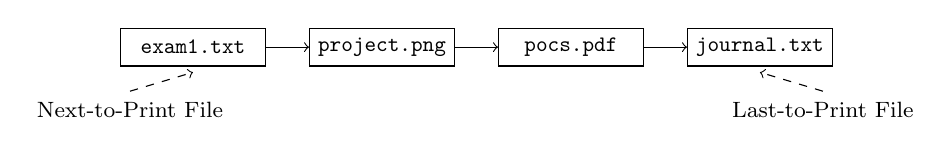
\begin{tikzpicture}[
    scale=.8,
  queuenode/.style={rectangle, draw, minimum width=1.5cm, minimum height=0.6cm, minimum width=2.3cm, text centered,scale=.8},
  dashedarrow/.style={->, dashed}
]

% Queue nodes
\node[queuenode] (front) at (0, 0) {\texttt{exam1.txt}};
\node[queuenode] (node1) at (3, 0) {\texttt{project.png}};
\node[queuenode] (node2) at (6, 0) {\texttt{pocs.pdf}};
\node[queuenode] (node3) at (9, 0) {\texttt{journal.txt}};

% Arrows
\draw[->] (front.east) -- (node1.west);
\draw[->] (node1.east) -- (node2.west);
\draw[->] (node2.east) -- (node3.west);

\draw[dashedarrow] (-1, -.7) -- (0, -.4);
\node[align=center] at (-1, -1) {\footnotesize{}Next-to-Print File};

\draw[dashedarrow] (10, -.7) -- (9, -.4);
\node[align=center] at (10, -1) {\footnotesize{}Last-to-Print File};

\end{tikzpicture}
\end{center}
\caption{Example of Printer Task Queue}
\label{fig:printerqueue}
\end{figure}

Unfortunately and inconveniently, there is no \ttt{Queue} class in Java. Instead, \texttt{Queue} is an \textit{interface}\index{interface} that other classes implement whose structure resembles a queue. To create a first-in-first-out queue data structure, we may initialize a variable to be a \texttt{Queue} then instantiate it as a \texttt{LinkedList}. Thankfully, the \texttt{LinkedList} class contains all relevant methods for operating a FIFO-based queue.
\begin{verbnobox}[\small]
Queue<Integer> q = new LinkedList<>();
\end{verbnobox}
Treating \texttt{q} as a queue rather than a linked list is easy thanks to the methods supplied by the \texttt{LinkedList} implementation. Figure~\ref{fig:queues} shows some of these handy methods. 
\begin{figure}[tp]
  \small
  \begin{tcolorbox}[title=Java Queue]
    A \textit{Queue} is a first-in-first-out (FIFO) sequential data structure where each element is linked to the element immediately after.
    \vspace{2ex}
  \begin{description}
    \item [\ttt{Queue<$T$> $Q=$ new LinkedList<>()}] creates a \ttt{Queue} of type $T$, named $Q$.
     \item [\ttt{$Q$.addLast$(e)$}] adds $e$ to the end of $Q$, placing it at the end of the queue structure.
     \item [\ttt{$Q$.poll$()$}] returns and removes the element from the front of the queue.
     \item [\ttt{$Q$.peek$()$}] returns the front-most element in the queue.
    \item [\ttt{$Q$.size$()$}] returns the number of logical elements in the queue.
  \end{description}
\end{tcolorbox}
  \caption{Useful \ttt{Queue}-based Methods.}
  \label{fig:queues}
\end{figure}

\subsubsection*{\ttt{PriorityQueue} Class}
\begin{figure}[tp]
  \small
  \begin{tcolorbox}[title=Java PriorityQueue]
    A \textit{Priority queue} is a rank/score-based data structure wherein the ordering of elements is determined by either their natural ordering or a \ttt{Comparator}.
    \vspace{2ex}
  \begin{description}
    \item [\ttt{Queue<$T$> $PQ=$ new PriorityQueue<>($c$)}] creates a \ttt{PriorityQueue} of type $T$, named $PQ$, with a \ttt{Comparator} $c$ that is used to compare objects of type $T$ within the priority queue.
     \item [\ttt{$PQ$.add$(e)$}] inserts $e$ into $PQ$, whose position in the priority queue depends on the currently-existing elements.
     \item [\ttt{$PQ$.poll$()$}] returns and removes the element with the highest priority.
     \item [\ttt{$PQ$.peek$()$}] returns the element with the highest priority.
    \item [\ttt{$PQ$.size$()$}] returns the number of logical elements in the priority queue.
  \end{description}
\end{tcolorbox}
  \caption{Useful \ttt{PriorityQueue}-based Methods.}
  \label{fig:priorityqueues}
\end{figure}

\textit{Priority queues} are the final sequential data structure that we will discuss from the Collections API\@. Though, placing it in this section is slightly disingenuous because, while priority queues have an ordering in their underlying data structure, saying that elements correspond to an index is largely incorrect. Priority queues, as their name suggests, rank items in the queue by a score called the \textit{priority}. Elements with the highest priority are at the ``front'' of the priority queue. Inserting elements into a priority queue potentially alters the positioning of preexisting elements.

Priority queues base priority on one of two contributing factors: either the \textit{natural ordering} of elements, or a \textit{comparator object}. The natural ordering of elements is straightforward: natural ordering for numbers is their standard numeric ordering. For strings, the natural ordering is by lexicographical ordering. These, however, are not as interesting as comparators, which we will now discuss.

A \textit{comparator} is a way of comparing two arbitrary ``things,'' whether these things are numbers (i.e., the wrapper classes), strings, or another kind of object, we can define custom ways of comparing \textit{any} non-primitive datatype.

\example{Let us design a \ttt{Comparator} for prioritizing strings that start with the lowercase letter \ttt{`p'}. Comparators are constructed like other objects via \ttt{new}, but something interesting about their implementation is that we must specify \textit{how} to compare two objects. Therefore when we create a new instance of \ttt{Comparator} we must also override its \ttt{compare} method. This method's signature varies based on the parameterized type provided to the comparator, but since we want to compare strings, we should declare it as follows:\footnote{Again, we are labeling the return type as a \textit{Queue} because priority queues are a type of queue. Upon instantiating a new priority queue, Java will typecheck the return value against the signature of the method to verify that we are returning something that is, in fact, a queue.}}

\begin{cl}[]{}
\begin{lstlisting}[language=MyJava]
import java.util.Comparator;
import java.util.PriorityQueue;
import java.util.Queue;

class PriorityQueueByP {

  /**
   * Returns a priority queue that prioritizes strings that start with `p'.
   * @return priority queue instance.
   */
  static Queue<String> priorityByP() {
    Comparator<String> c = new Comparator<>(
      @Override
      public int compare(String s1, String s2) { 
        // TODO.
      }
    );
  }
}
\end{lstlisting}
\end{cl}

We now must specify how to compare \ttt{s1} and \ttt{s2} to achieve our goal. Strangely enough, if we want to say that \ttt{s1} has a higher priority than \ttt{s2}, we must return a negative value, similar to the natural ordering of strings (this idea extends to any type we wish to compare, however). So, we perform a case analysis on the strings. If both strings are non-empty, we grab their first character. If both start with `p', then their ordering depends on a standard lexicographical comparison of the rest of the strings. If the first character of $s_1$ is `p', however, we return $-1$ to designate that $s_1$ has a higher priority than $s_2$. Conversely, if $s_2$ starts with `p', then we return $1$ to designate the opposite. If neither start with $p$, then again we perform a lexicographical comparison on the entire strings. Algorithm~\ref{alg:pseudocodepriority} displays the pseudocode for the comparator, but as we will see, we can translate this, verbatim, into Java syntax. The last line of \ttt{priorityByP} instantiates a new \ttt{PriorityQueue} whose constructor receives the \ttt{Comparator} that we just designed. 
\begin{algorithm}[H]
\begin{algorithmic}
\Procedure{Compare}{$s_1$, $s_2$}
    \If {$s_1$ \textbf{and} $s_2$ are non-empty}
        \State $c_1 \gets \textbf{First}(s_1)$
        \State $c_2 \gets \textbf{First}(s_2)$
        \If {$c_1$ is `p' \textbf{and} $c_2$ is `p'}
            \State $xs_1 \gets s_1$\textit{.substring(1)}
            \State $xs_2 \gets s_2$\textit{.substring(1)}
            \State \Return $xs_1$\textit{.compareTo}$(xs_2)$
        \ElsIf {$c_1$ is `p'}
            \State \Return $-1$
        \ElsIf {$c_2$ is `p'}
            \State \Return $1$
        \Else
            \State \Return $s_1$\textit{.compareTo}$(s_2)$
        \EndIf
    \Else
        \State \Return $s_1$\textit{.compareTo}$(s_2)$
    \EndIf
\EndProcedure
\end{algorithmic}
\caption{Pseudocode for Comparing Two Strings For `p' Priority}
\label{alg:pseudocodeinsertion}
\end{algorithm}

\begin{cl}[]{}
\begin{lstlisting}[language=MyJava]
import java.util.Comparator;
import java.util.PriorityQueue;
import java.util.Queue;

class PriorityQueueByP {

  static Queue<String> priorityByP() {
    Comparator<String> c = new Comparator<>(
      @Override
      public int compare(String s1, String s2) {
        if (!s1.isEmpty() && !s2.isEmpty()) {
          char c1 = s1.charAt(0);
          char c2 = s2.charAt(0);
          if (c1 == 'p' && c2 == 'p') {
            return s1.substring(1).compareTo(s2.substring(1));
          } else if (c1 == 'p') {
            return -1;
          } else if (c2 == 'p') {
            return 1;
          } else {
            return s1.compareTo(s2);
          }
        } else {
          return s1.compareTo(s2);
        }
      }
    );

    return new PriorityQueue<String>(c);
  }
}
\end{lstlisting}
\end{cl}

Let us add a few elements to a priority queue with our custom comparator to exemplify the idea. To add elements, we use \ttt{.add}, and to remove the element with the highest priority, we invoke \ttt{.poll}.

\begin{cl}[]{}
\begin{lstlisting}[language=MyJava]
import java.util.Comparator;
import java.util.PriorityQueue;
import java.util.Queue;

class PriorityQueueByP {

  static Queue<String> priorityByP() {
    // Implementation not shown.
  }

  public static void main(String[] args) {
    Queue<String> pq1 = priorityByP();
    // Add a few values.
    pq1.add("pool");
    pq1.add("peek");
    pq1.add("hello");
    pq1.add("barks");
    pq1.add("park");
    pq1.add("pecking");
    pq1.add("shrub");

    // Poll each from the queue.
    while (!pq1.isEmpty()) {
      System.out.println(pq1.poll());
    }
  }
}
\end{lstlisting}
\end{cl}
The output is as follows:
\begin{verbnobox}[\small]
park
pecking
peek
pool
barks
hello
shrub
\end{verbnobox}
Why is this what the priority queue outputs? If we reason about this with our comparator, it becomes clear. \ttt{park} has the highest priority because it starts with `p' and has a substring that comes before the rest of those strings starting with `p'. The strings \ttt{pecking}, \ttt{peek}, and \ttt{pool} come next for similar reasons. Finally, none of the strings \ttt{barks}, \ttt{hello}, and \ttt{shrub} start with `p', so we simply compare based on the strings themselves. The underlying implementation of how the priority queue works is beyond the scope of this textbook. These details are generally reserved for a textbook or course on advanced data structures, which follows the course designed for the audience of this text.

\subsection*{Set-Based Data Structures}
\textit{Sets} are unordered collections of non-duplicate elements. Does this definition sound familiar? It should; it perfectly mirrors the mathematical definition of a set. Java has a few nuances to its definition of sets that we will now see. We consider these data structures \textit{set-based} since they all rely on the ``no-duplicate'' philosophy.

\subsubsection*{\ttt{Set} Interface}
A \textit{Set} in Java is an interface rather than a class. This is because Java has a hierarchy for differing implementations of sets. We will discuss three: \textit{HashSet}, \textit{TreeSet}, and \textit{LinkedHashSet}. While all three disallow duplicate elements, the latter two impose an ordering on their elements, which goes against the standard mathematical definition, but for practical reasons.

\subsubsection*{\ttt{HashSet} Class}
The \textit{HashSet} implementation of sets determines existence of objects in the set by the \textit{hashcode} of the object. Recall that we can think of hashcodes as an association for objects. In fact, in our discussion on strings and arrays, a comparison using \ttt{==} compares the hashcodes of the objects to see if they are identical, rather than containing the same content.
 Hash sets are convenient and fast to work with due to the underlying implementation, whose details are beyond the scope of this text. Use hash sets when you do not care about element ordering or ``position'' in the set, but want to ensure no duplicates exist.
\begin{figure}[tp]
  \small
  \begin{tcolorbox}[title=Java Hash Sets]
    A \textit{HashSet} is a set of non-duplicate elements with no defined ordering. Elements are inserted into the set by their hashcode.
    \vspace{2ex}
  \begin{description}
    \item [\ttt{Set<$T$> $S=$ new HashSet<>()}] creates a \ttt{HashSet} of type $T$, named $S$.
     \item [\ttt{$S$.contains$(e)$}] returns whether or not $e$ is in the set $S$.
     \item [\ttt{$S$.add$(e)$}] adds $e$ to the set $S$ only if it is not present. If $e$ is in $S$, nothing happens.
     \item [\ttt{$S$.remove$(e)$}] removes $e$ from the set $S$ only if it is present. If $e$ is not in $S$, it returns \ttt{false}; otherwise, it returns \ttt{true}.
    \item [\ttt{$S$.size$()$}] returns the number of logical elements in the set.
  \end{description}
\end{tcolorbox}
  \caption{Useful \ttt{HashSet}-based Methods.}
  \label{fig:hashsets}
\end{figure}

\subsubsection*{\ttt{TreeSet} Class}
A \textit{TreeSet} is a set with a determined order, either by a natural ordering or that defined by a \ttt{Comparator}, like a priority queue. All methods in a \ttt{Set} are implemented by a \ttt{TreeSet}. Those listed from the \ttt{HashSet} figure are also implemented.

\subsubsection*{\ttt{LinkedHashSet} Class}
A \textit{LinkedHashSet} is a set with an ordering based on the insertion order of the elements. All methods in a \ttt{Set} are implemented by a \ttt{LinkedHashSet}. Those listed from the \ttt{HashSet} figure are also implemented.

\subsection*{Dictionary-Based Data Structures}
Dictionaries maps elements from one type $K$ to elements of another type $V$. These types $K$ and $V$ do not necessarily need to be distinct. 

\subsubsection*{\ttt{Map} Interface}
Java has an interface called \ttt{Map} rather than a class because, like sets, there is a hierarchy for differing implementations of maps. We will discuss three: \textit{HashMap}, \textit{TreeMap}, and \textit{LinkedHashMap}. Maps contain keys and values; the keys are mapped to values in the map. Additionally, maps cannot contain duplicate keys.

\subsubsection*{\ttt{HashMap} Class}
\textit{HashMaps} base existence of keys in the map by their hashcode, identical to a HashSet. 
\begin{figure}[tp]
  \small
  \begin{tcolorbox}[title=Java Hash Maps]
    A \textit{HashMap} is a dictionary-based data structure wherein we map \textit{keys} to \textit{values}. The position of these pairs in the map is according to the hashcode of the key.
    \vspace{2ex}
  \begin{description}
    \item [\ttt{Map<$K, V$> $M=$ new HashMap<>()}] creates a \ttt{HashMap} named $M$ whose keys are of type $K$ and whose values are of type $V$. Namely, the keys map to the values.
     \item [\ttt{$M$.containsKey$(k)$}] returns whether or not $k$ is a key in the map $M$.
     \item [\ttt{$M$.put$(k, v)$}] maps the key $k$ to the value $v$ in $M$.
     \item [\ttt{$M$.get$(k)$}] returns the value associated with $k$ in $M$, or \ttt{null} if $k$ does not have a mapping.
    \item [\ttt{$S$.size$()$}] returns the number of logical elements in the set.
  \end{description}
\end{tcolorbox}
  \caption{Useful \ttt{HashMap}-based Methods.}
  \label{fig:hashmap}
\end{figure}

\subsection*{\ttt{TreeMap} Class}
A \textit{TreeMap} is a map with a determined order, either by a natural ordering of the keys or that defined by a comparator. All method sin a \texttt{Map} are implemented by a \texttt{TreeMap}.

\subsection*{\ttt{LinkedHashMap} Class}
A \textit{LinkedHashMap} is a map with an ordering based on the insertion order of the key/value pairs. All methods in a \ttt{Map} are implemented by a \ttt{LinkedHashMap}. Those listed from the \ttt{HashMap} figure are also implemented.

\section*{Iterators}
We know how to iterate, or traverse, over a simple data structure, e.g., an array. The idea is to use an index and continuously increment the index until we are at the end bounds of the array. Below is a simple example of summing the elements of an array, which we have seen repeatedly by now.

\begin{verbnobox}[\small]
static int sum(int[] arr) {
  int sum = 0;
  for (int i = 0; i < arr.size; i++) { sum += arr[i]; }
  return sum;
}
\end{verbnobox}

The problem is that not all data structures, as we have undoubtedly seen, are sequential; sets and maps are two examples of non-sequential data structures, so how do we traverse over those? Stacks and queues are another example of data structures that are not necessarily sequential. \textit{Iterator} objects are the answer to this problem. Iterators provide a mechanism for traversing over a generalized data structure. Any data structure whose class definition implements \ttt{Iterator} must define at least two methods: \ttt{boolean hasNext} and \ttt{T next}, which determines whether or not we are at the end of the traversal and retrieves the next element respectively. Note that \ttt{T}, for the time being, simply means ``any type.'' All of the Java collections implement \ttt{Iterator}, we can retrieve the corresponding \ttt{Iterator} object via the \ttt{.iterator} method. 

Upon retrieving an iterator, we can use a \ttt{while} loop to continuously traverse over the data structure until no more elements remain to be visited. The elements of the iterator are generated on-the-fly; only upon calling \ttt{next} is the value truly read from the data structure itself. Much like the rest of the Collections API, we must pass the parameterized type to the \ttt{Iterator} initialization so that it knows what to substitute for \ttt{T} in the \ttt{next} method.

\example{Let's use an iterator to traverse over a \ttt{LinkedHashSet}, whose elements ordering is determined by their insertion order, meaning the iterator should produce them in the order in which they were inserted.}

\begin{cl}[]{Testing an Iterator over a \ttt{LinkedHashSet}}
\begin{lstlisting}[language=MyJava]
import static Assertions.assertAll;
import static Assertions.assertEquals;

import java.util.Set;
import java.util.LinkedHashSet;
import java.util.Iterator;

class IteratorTester {

  @Test
  void testIterator() {
    Set<Integer> lhs = new LinkedHashSet<>();
    lhs.add(8);
    lhs.add(10);
    lhs.add(0);
    lhs.add(90);
    Iterator<Integer> it = lhs.iterator();
    assertAll(
      () -> assertTrue(it.hasNext());
      () -> assertEquals(8, it.next()),
      () -> assertEquals(10, it.next()),
      () -> assertEquals(0, it.next()),
      () -> assertEquals(90, it.next()),
      () -> assertFalse(it.hasNext()));
  }
} 
\end{lstlisting}
\end{cl}

Should we want to traverse over the data again, we need to produce yet another instance of the iterator because there is no way to reset the ``position'' of an iterator; they are a type of one-time use objects.

It should be stated that the enhanced \ttt{for} loop is nearly identical to the job of an \ttt{Iterator}, so a programmer may wonder why not use the former over the latter. Inside an enhanced \ttt{for} loop, we cannot modify the data structure, meaning that we cannot add, insert, remove, or change elements. On the other hand, iterators allow structural modification. We would not recommend altering the data structure, even if it is permissible by Java, since doing so can result in irksome bugs. 

\example{Let's now iterate over the \ttt{LinkedHashSet} using an enhanced \ttt{for} loop. We can do so by placing the type on the left-hand side of the element declaration. Our test will simply subtract the elements from left-to-right, since subtraction is not commutative, we can quickly verify the correctness of our result.}

\begin{cl}[]{Using an Enhanced \ttt{for} Loop over a Collection}
\begin{lstlisting}[language=MyJava]
import static Assertions.assertEquals;

import java.util.Set;
import java.util.LinkedHashSet;

class EnhancedForLoopTester {

  @Test
  testEnhancedForLoop() {
    Set<Integer> lhs = new LinkedHashSet<>();
    lhs.add(1);
    lhs.add(2);
    lhs.add(3);
    lhs.add(4);
    int diff = 0;
    for (Integer e : lhs) { diff -= e; }
    assertEquals(-10, diff);
  }
}
\end{lstlisting}
\end{cl}

\section*{Streams}
\textit{Streams} are, in effect, a \textit{lazy} collection of ``things.'' By lazy, we mean to say that, if a result is not necessary, or requested, then it is not computed.

\example{Consider a situation in which we invoke a method called \ttt{omega()}, which is defined as an infinite loop, as the argument to the \ttt{foo} method, giving us \ttt{foo(omega())}. In Java, all arguments are evaluated \textit{eagerly}, which means that, in effect, takes an eternity to terminate. Unfortunately for the caller of \ttt{foo}, we do not even use the value of $x$, meaning we computed \ttt{omega()} for absolutely no reason whatsoever. This means that, because \ttt{omega} never terminates, \ttt{foo} similarly never returns a result.} 

\begin{verbnobox}[\small]
static int omega() {
  while (true) {}
  return 10;
}
\end{verbnobox}
\begin{verbnobox}[\small]
static int foo(int x) {
  return 5;
}
\end{verbnobox}

If Java supported \textit{lazy evaluation} for method calls, we would not be in this predicament. Our discussion is not entirely driven by a desire for lazy evaluation, but rather the desire for easily-composable operations; lazy evaluation is a perk in that it allows us to design infinite data structures! An ``infinite'' data structure raises some important questions about how to store ``infinite'' data. Imagine that we want to compute a list that contains every positive even integer. We can represent this as the following inductive set:
\begin{align*}
    &0 \in S\\
    &\text{If } x \in S,\text{ then }x + 2 \in S
\end{align*}
Therefore $S$ is a set containing countably-infinite values. Implementing $S$ in Java, as an \ttt{ArrayList}, might contain a \ttt{for} loop with a condition that we do not know how to solve! In this case, since we do not know how many values to add, we might design an infinite loop via \ttt{while (true)}, but then the loop never ends. Eventually the program runs out of memory due to adding values to the never-ending list. The solution, as we have suggested, is to use streams.\footnote{For those coming from another language such as Python, a stream is equivalent to a \textit{generator}.}

To create a stream of infinite data is to recreate our inductive set definition inside a \ttt{IntStream} instance and the \ttt{iterate} static method.

\begin{verbnobox}[\small]
IntStream is = IntStream.iterate(0, x -> x + 2);
\end{verbnobox}

Let us explain this method, but to do so we must introduce \textit{lambda expressions}. A lambda expression is an anonymous function, i.e., a function definition without a name. In the above code snippet, we define a function that receives a value $x$ and returns $x$ plus two. It would be identical to defining a \ttt{private static} method to add two to some integer, but we like lambda expressions due to their locality; it might come across as superfluous to design a method that is used in only one context. Should we want to pass a method reference instead of a lambda expression, this is easily attainable.
\begin{cl}[]{}
\begin{lstlisting}[language=MyJava]
import java.util.IntStream;

class PositiveEvens {

  private static int addTwo(int x) { return x + 2; }

  public static void main(String[] args) {
    IntStream is = IntStream.iterate(0, PositiveEvens::addTwo);
  }
}   
\end{lstlisting}
\end{cl}

The \ttt{IntStream} instance declares a stream that, when requested/prompted, invokes and populates the stream. Because it is impossible to represent an infinite data structure in Java with modern computers, we should limit how many values we want from this stream. Indeed, the \ttt{.limit} method computes exactly $n$ elements from the stream. So, to compute the first ten elements of our $\textit{is}$ \ttt{IntStream}, we invoke \ttt{.limit(10)} on our $\textit{is}$ stream. 

\begin{cl}[]{}
\begin{lstlisting}[language=MyJava]
import java.util.IntStream;

class PositiveEvens {
  
  public static void main(String[] args) {
    IntStream is = IntStream.iterate(0, x -> x + 2).limit(10);
  }
}
\end{lstlisting}
\end{cl}
Now, suppose we want to view these ten elements. Right now they are consolidated into an \ttt{IntStream}, but we need to convert them to a list of sorts. The solution is to convert the values into a \ttt{Stream<Integer>} via \ttt{.boxed()}, and then to a list using the convenient \ttt{.toList()} method.
\begin{cl}[]{}
\begin{lstlisting}[language=MyJava]
import java.util.IntStream;
import java.util.List;

class PositiveEvens {
  
  public static void main(String[] args) {
    IntStream is = IntStream.iterate(0, x -> x + 2).limit(10);
    List<Integer> ls = is.boxed().toList();
    System.out.println(ls); // [0, 2, 4, 6, 8, 10, 12, 14, 16, 18]
  }
}
\end{lstlisting}
\end{cl}

\example{Suppose we want a stream of infinitely repeating \ttt{"a"} strings. We can easily do this via the \ttt{generate} method, which acts as the stream constructor, receiving a lambda expression to continuously generate new elements.}
\begin{cl}[]{}
\begin{lstlisting}[language=MyJava]
import java.util.Stream;

class AGenerator {

  public static void main(String[] args) {
    Stream<String> as = Stream.generate(() -> "a");
    // ["a", "a", "a", "a", "a", "a", "a", "a", "a", "a"]
    System.out.println(as.limit(10).boxed().toList()); 
  } 
}
\end{lstlisting}
\end{cl}

Again, it is important to understand what is going on under the hood of a stream. Elements thereof only generate when we request them through some accessory means, e.g., \ttt{limit}. As we previously suggested, attempting to access an infinite stream without a limit causes the program to hang and eventually crash with an \ttt{OutOfMemoryError} exception.

\example{Imagine we want to create a stream of all of the Fibonacci numbers. The thing is, eventually we will reach the $32$-bit limit for the \ttt{int} datatype, so we should take advantage of the \ttt{BigInteger} class, which allows us to represent arbitrarily-large integers.\footnote{Worrying about \textit{how} the \ttt{BigInteger} class works for now is unnecessary as our current plan is to demonstrate stream properties.} Also, this time we will write a method that returns the stream instance rather than creating it in the \ttt{main} method.}

Here's what we need to do: we will use \ttt{iterate} to generate new values in the sequence. There is a slight problem in that the Fibonacci sequence has two starting (accumulator) values: $0$ and $1$. The issue is that \ttt{iterate} receives only one ``initializer'' value. To circumvent this predicament we can simply pass an array that contains the current and ``next'' Fibonacci values. Inside the lambda expression we of course receive an array of values, from which we can compute the next Fibonacci number. This time, however, instead of using \ttt{IntStream}, we will generalize to the \ttt{Stream} class since our initial value(s) is not an integer.

\begin{cl}[]{}
\begin{lstlisting}[language=MyJava]
import static Assertions.assertEquals;

import java.util.Stream;
import java.util.List;
import java.util.ArrayList;
import java.util.BigInteger;

class BigIntFibStreamTester {

  @Test
  void bigIntFibStreamTest() {
    // Get the stream, test ten values, make sure the lists are the same
    // length, then test each subarray.
    Stream<BigInteger[]> s = StreamExample.fibonacciStream();
    List<BigInteger[]> actualLs = s.limit(10).toList();
    List<BigInteger[]> expectedLs 
      = new ArrayList<>(
        List.of(new BigInteger[]{new BigInteger("0"), new BigInteger("1")},
                new BigInteger[]{new BigInteger("1"), new BigInteger("1")},
                ...));

    // Check each array of BigIntegers of the expected and actual.
    assertTrue(expectedLs.size() == actualLs.size());
    for (int i = 0; i < expectedLs.size(); i++) {
      assertArrayEquals(expectedLs.get(i), actualLs.get(i));
    }
  }
}
\end{lstlisting}
\end{cl}

\begin{cl}[]{}
\begin{lstlisting}[language=MyJava]
import java.util.Stream;
import java.util.BigInteger;

class BigIntFibStream {

  /**
   * Computes a stream of BigInteger values computing the nth Fibonacci value.
   * @return stream containing arrays of the next sequential BigIntegers.
   */
  static Stream<BigInteger[]> fibonacciStream() {
    BigInteger[] vals = new BigInteger[]{new BigInteger("0"), 
                                         new BigInteger("1")};
    return Stream.iterate(vals, v -> new BigInteger[]{v[1], v[0].add(v[1])});
  }
}
\end{lstlisting}
\end{cl}

\begin{figure}[tp]
  \small
  \begin{tcolorbox}[title=Java Streams]
    A \textit{stream} is a lazy collection of elements that are computed only when requested.
    \vspace{2ex}
  \begin{description}
    \item [\ttt{int $S$.count$()$}] returns the number of elements in the stream.
    \item [\ttt{Stream<$T$> $S$.map($f$)}] returns a new stream whose elements are the result of applying $f$ to each element of $S$.
    \item [\ttt{Stream<$T$> $S$.filter($p$)}] returns a new stream of values in $S$ that satisfy the predicate $p$.
    \item [\ttt{Stream<$T$> $S$.reduce($a$, $f$)}] returns the result of applying the binary function $f$ to each element of $S$, starting from $a$, which serves as the accumulator's initial value.
    \item [\ttt{Stream<$T$> $S$.limit($n$)}] returns a new stream containing the first $n$ elements of $S$.
    \item [\ttt{Stream<$T$> $S$.skip($n$)}] returns a new stream containing the elements of $S$ after the first $n$.
    \item [\ttt{Optional<$T$> $S$.min/max($c$)}] returns the minimum/maximum element of $S$ according to the comparator $c$. If $S$ is empty, returns \ttt{Optional.empty()}.
  \end{description}
\end{tcolorbox}
  \caption{Useful \ttt{Stream}-based Methods.}
  \label{fig:streams}
\end{figure}

\begin{figure}[tp]
  \small
  \begin{tcolorbox}[title=Java Stream--Searching Methods]
    We can search for the existence of types of elements in a stream.
    \vspace{2ex}
  \begin{description}
    \item [\ttt{boolean $S$.anyMatch($p$)}] returns \ttt{true} if \textbf{at least one} element of $S$ satisfies the predicate $p$; otherwise, returns \ttt{false}.
    \item [\ttt{boolean $S$.allMatch($p$)}] returns \ttt{true} if \textbf{all} elements of $S$ satisfy the predicate $p$; otherwise, returns \ttt{false}.
    \item [\ttt{boolean $S$.noneMatch($p$)}] returns \ttt{true} if \textbf{no} elements of $S$ satisfy the predicate $p$; otherwise, returns \ttt{false}.
  \end{description}
\end{tcolorbox}
  \caption{Useful \ttt{Stream}-Searching Methods.}
  \label{fig:streams-searching}
\end{figure}

So our code now produces a list of \ttt{BigInteger} arrays containing the current Fibonacci value and its successor. Though, is this really what we want? A better solution would be to simply return the first element of the tuple/two-element array. We can achieve this via the \ttt{map} function. \ttt{map} receives a lambda expression as an argument and applies it to every element of the acting stream. Let's modify the code a bit to see an improved output. Excellently, this change means we do not need to loop over our expected/actual lists in the unit testing method, as \ttt{assertEquals} works as intended over \ttt{List} objects.

\begin{cl}[]{}
\begin{lstlisting}[language=MyJava]
import static Assertions.assertEquals;

import java.util.Stream;
import java.util.List;
import java.util.ArrayList;
import java.util.BigInteger;

class BigIntFibStreamTester {

  @Test
  void testBigIntFibStream() {
    Stream<BigInteger> s = StreamExample.fibonacciStream();
    List<BigInteger> actualLs = s.limit(10).toList();
    List<BigInteger[]> expectedLs 
      = new ArrayList<>(
        List.of(new BigInteger[]{new BigInteger("0"), new BigInteger("1")},
                new BigInteger[]{new BigInteger("1"), new BigInteger("1")},
                ...));
    assertEquals(expectedLs, actualLs);
  }
}
\end{lstlisting}
\end{cl}

\begin{cl}[]{}
\begin{lstlisting}[language=MyJava]
import java.util.Stream;
import java.util.BigInteger;

class BigIntFibStream {

  /**
   * Computes a stream of BigInteger values computing the nth Fibonacci value.
   * @return stream containing arrays of the next sequential Fibonacci BigIntegers.
   */
  static Stream<BigInteger> fibonacciStream() {
    BigInteger[] vals = new BigInteger[]{new BigInteger("0"),
                                         new BigInteger("1")};
    return Stream.iterate(vals, v -> new BigInteger[]{v[1], v[0].add(v[1])})
                 .map(v -> v[0]);
  }
}
\end{lstlisting}
\end{cl}

We will now take a bit more of a look at \ttt{map}, as well as other useful \textit{higher-order functions} such as \ttt{filter} and \ttt{reduce}.

A \textit{higher-order function} is a function that takes functions as parameters. We saw that \ttt{map} receives a lambda expression and applies it to every element of a stream. 

\example{Let's write the \ttt{sqList} method that receives a \ttt{List<Integer>} and squares each element using the Stream API. The method should return a new list. A motif presented throughout stream methods is that they do not modify the original data. We should use \ttt{map} to apply a lambda expression that receives an integer and returns its square. Fortunately for us, we can convert any collection into a stream using the \ttt{.stream()} method. From there, we use a simple \ttt{map} invocation to arrive at our desired outcome.}

\begin{cl}[]{}
\begin{lstlisting}[language=MyJava]
import static Assertions.assertAll;
import static Assertions.assertEquals;
import static SqList.sqList;

import java.util.List;
import java.util.ArrayList;

class SqListTester {

  @Test
  void sqListTest() {
    List<Integer> ls1 = new ArrayList<>(List.of(1, 4, 9, 16, 25));
    List<Integer> ls2 = new ArrayList<>(List.of(0, 100, 81, 81));
    List<Integer> ls3 = new ArrayList<>();
    assertAll(
      () -> assertEquals(ls1, sqList(new ArrayList<>(List.of(1, 2, 3, 4, 5)))),
      () -> assertEquals(ls2, sqList(new ArrayList<>(List.of(0, 10, 9, 9)))),
      () -> assertEquals(ls3, sqList(new ArrayList<>())));
  }
}
\end{lstlisting}    
\end{cl}

\begin{cl}[]{}
\begin{lstlisting}[language=MyJava]
import java.util.List;

class SqList {

  /**
   * Returns a list of squared integers from a list of integers.
   * @param list of integers.
   * @return list of squared integers.
   */
  static List<Integer> sqList(List<Integer> ls) {
    return ls.stream()
             .map(x -> x * x)
             .toList();
  }
}
\end{lstlisting}    
\end{cl}

\example{Now, let's write the \ttt{removeVowels} method, which receives a string and removes all vowels, returning a new string in the process. This requires a few techniques that we have learned, but also means we need to use \ttt{filter} and \ttt{reduce}. Here's the idea:}

\begin{enumerate}
    \item Convert the given \ttt{String} into a stream of integers representing the ASCII values of characters.
    \item Convert each integer to a ``one-string,'' i.e., a \ttt{String} of one character. The reasoning behind this decision will become clear later.
    \item Filter out vowels from the stream.
    \item Accumulate the characters in a new string.
\end{enumerate}

Of course, we begin by writing a few tests. Fortunately, writing tests is simple for this method, whereas the implementation is the most complex seen thus far.

\begin{cl}[]{Tests for \ttt{removeVowels} Method}
\begin{lstlisting}[language=MyJava]
import static Assertions.assertAll;
import static RemoveVowelsStream.removeVowels;

class RemoveVowelsStreamTester {
  
  @Test
  void testRemoveVowels() {
    assertAll(
      () -> assertEquals("hll", StreamTests.removeVowels("hello")),
      () -> assertEquals("hw r y?", StreamTests.removeVowels("how are you?")),
      () -> assertEquals("", StreamTests.removeVowels("aaaaaaaaaaaa")),
      () -> assertEquals("bbbbbbbbbb", StreamTests.removeVowels("bbbbbbbbbb")),
      () -> assertEquals("bbbbb", StreamTests.removeVowels("abababababa")),
      () -> assertEquals("hll", StreamTests.removeVowels("aeiouAEIOU")));
  }
}
\end{lstlisting}
\end{cl}

Onto the definition; we start by writing the method signature and purpose. Then, we need to complete step one: convert the given string into a stream of ASCII integers, which is achievable via the \ttt{.chars} method. It returns an \ttt{IntStream} of integer ASCII values. Step two involves us converting each integer into a ``one-string,'' which we can do via the constructor for a \ttt{String} object. Step three requires the use of \ttt{filter}, which is another higher-order function. It receives a lambda expression and returns those objects from the stream that satisfy the filter. Since we want to filter \textit{out} the vowels, we should write a method that determines if a character is vowel, then negate the expression as part of the lambda definition. Lastly we arrive at accumulating the characters into a new string, requiring us to use \ttt{reduce}: yet another higher-order function. The reduce function receives an initial value, i.e., an accumulator $a$ and a binary function $f$. It then applies the binary function to each value in the stream and the running accumulator. If this reminds you of tail recursion, then indeed, that is exactly how reduce works; It folds over the list/stream of values, building the result in the accumulator variable.\footnote{In other functional programming languages, \ttt{reduce} is commonly called \ttt{foldr}.} Due to the simplicity of the \ttt{isVowel} predicate and its implementation in Chapter~\ref{chapter-crl}, we omit its definition.

\begin{cl}[]{Definition of \ttt{removeVowels} Using Streams}
\begin{lstlisting}[language=MyJava]
class RemoveVowelsStream {

  /**
   * Removes all vowels from a given string using streams.
   * @param s - string to remove vowels from.
   * @return new string.
   */
  static String removeVowels(String s) {
    return s.chars()
            .mapToObj(c -> String.valueOf(c))
            .filter(c -> !isVowel(c))
            .reduce("", (acc, c) -> acc + c);
  }
}
\end{lstlisting}
\end{cl}

\subsubsection*{Optional Type}
The primary benefit of streams is their compositionality. We can chain together multiple operations, sequentially, to compute a result. Though, there are instances in which a value may not exist, and the stream has to account for these somehow.

\example{Consider a series of stream operations to find the maximum integer of a list. For the general case, this is straightforward, but what about when the list is empty? It does not make sense to return zero, since the maximum integer in a list may very well be zero, which leads to a false conclusion. The solution, in this case, is the \ttt{Optional} class. An \ttt{Optional} is a container that may or may not contain a value. If so, we may access the value directly via \ttt{.get}. If we do not know whether or not it contains a value, we may use \ttt{.orElse($t$)}, which returns the encapsulated value if it exists, or $t$ otherwise. We can also check, prior to a retrieval, if the \ttt{Optional} contains a value via the \ttt{.isPresent} method. \ttt{Optional} is generic and works over any class type, like almost all other classes from the collections API. To test the return value of a stream operation that returns an \ttt{Optional}, e.g., \ttt{max}, we instantiate an \ttt{Optional} that wraps the resulting value if it exists, or \ttt{Optional.empty()} otherwise.}

\begin{cl}[]{Using the Optional Wrapper Class}
\begin{lstlisting}[language=MyJava]
import static Assertions.assertAll;
import static Assertions.assertEquals;

import java.util.Optional;
import java.util.List;

class OptionalTester {

  private static final List<Integer> LS1 = List.of(10, 20, 42, 12, 5);
  private static final List<Integer> LS2 = List.of();

  @Test
  void testMaxValue() {
    Optional<Integer> op1 = Optional.of(42);
    Optional<Integer> op2 = Optional.empty();
    assertAll(
      () -> assertEquals(op1, LS1.stream().max((a, b) -> a - b)),
      () -> assertEquals(op2, LS2.stream().max((a, b) -> a - b)),
      () -> assertEquals(42, LS1.stream().max((a, b) -> a - b).orElse(null));
      () -> assertNull(LS2.stream().max((a, b) -> a - b).orElse(null)));
  }
}
\end{lstlisting}
\end{cl}

Optional values, like we stated, work wonders with the compositionality of streams; if a value does not exist, the stream API will propagate an \ttt{empty} instance of \ttt{Optional} up the chain rather than displaying an error or crashing the program. As part of the design philosophy of the class, those decisions, i.e., whether to crash the program or not, remain a choice left for the implementing programmer.